%% Do not change document class, margins, fonts, etc.
\documentclass[a4paper,oneside,bibliography=totoc]{scrbook}

% some useful packages (add more as needed)
\usepackage[utf8]{inputenc}
\usepackage{graphicx}
\usepackage{latexsym}
\usepackage{amsmath}
\usepackage{amssymb}
\usepackage{subcaption}
\usepackage{tabularx}
\usepackage{booktabs}
\usepackage{algorithm} % you can modify the algorithm style to your liking
\counterwithin{algorithm}{chapter} % so that algorithms have chapter numbers as well
\usepackage{algorithmic}
\usepackage{csquotes}
\renewcommand{\algorithmiccomment}[1]{\hfill\textit{// #1}}
\usepackage[usenames,dvipsnames]{xcolor}
\usepackage[colorlinks,citecolor=Green]{hyperref} % you may change/remove the colors
\usepackage{lipsum} % you do not need this
\usepackage{tikz}
\usepackage{hyperref}
\newcommand{\bref}[1]{\hyperref[#1]{[\ref*{#1}]}}

% chicago citation style
\usepackage{natbib}
\bibliographystyle{chicagoa}
\setcitestyle{authoryear,round,semicolon,aysep={},yysep={,}} \let\cite\citep

% example enviroments (add more as needed)
\newtheorem{definition}{Definition} \newtheorem{proposition}{Proposition}

\begin{document}


% Quick fix to remove the 0 in front of sections.
\makeatletter
\renewcommand\thesection{\arabic{section}}
\renewcommand\thesubsection{\arabic{section}.\arabic{subsection}}
\renewcommand\thesubsubsection{\arabic{section}.\arabic{subsection}.\arabic{subsubsection}}
\makeatother

\frontmatter 
\pagenumbering{arabic} % Switch to Arabic numbering in the front matter
\subject{Project Report} % change to appropriate type
\title{Multi-Agent Gaming \\with the Board Game Diplomacy}
\author{
  Maxim Fröhlich (2266015)\\
  Gabriel Himmelein (1649181)\\
  David Siregar (2262617)\\
  Anatole Lobenko (2187322)\\
  José David Burbano Pesántez (2266830)
} \date{May 17, 2026}
\publishers{{\small Submitted to}\\
  Data and Web Science Group\\
  Dr. Ralph Peters\\
  Prof. Dr. Christian Bizer\\
  University of Mannheim\\}
\maketitle
\clearpage

\section{Application Area and Goals}
Large language models (LLMs) are typically evaluated on complex question answering and logical reasoning. However, these benchmarks fail to capture multi-agent challenges like negotiation, collaboration, and strategic planning. We addressed this gap by using the board game \texttt{Diplomacy} to investigate LLM behavior in a competitive social environment.

By assigning each of the seven \texttt{Diplomacy} powers to a different LLM agent, we forced them to build partnerships, communicate, and develop long-term tactics. This setup provided a robust evaluation environment for studying trust development, strategic decision-making, and time-based adaptation.

Our main objective was to evaluate LLM performance in long-horizon multi-agent settings. Specifically, we investigated whether agents enhanced their performance across games using context, long-term memory, and strategic adaptation to opponents' play styles. Thus, we explored memory and social reasoning as key determinants in negotiation-based environments.

\section{Profile of Data and Tasks}

\subsection{Data Sources}
Our project used self-generated simulation data rather than a traditional external dataset. Data originated from the \texttt{Diplomacy} engine during matches between seven LLM agents. We utilized structured game data (board states, supply centers), interaction data (negotiation messages, submitted orders), and agent-level context (diary summaries, memory records, and execution traces).

\subsection{Data Collection}
We collected data through controlled experiments varying model assignments and memory settings. Analyzing the resulting records yielded metrics like move success, territorial growth, and alliance behavior, allowing us to assess how different configurations impacted strategic performance over time.

\section{Approaches to Solving the Problem with LLM Agents}

\subsection{LLM Selection}

We built on a fork of the open-source \href{https://github.com/GoodStartLabs/AI_Diplomacy}{GoodStartLabs/AI\_Diplomacy} repository, which wrapped the \texttt{Diplomacy} game engine with an LLM agent system. The codebase's unified \texttt{BaseModelClient} interface allowed each of the seven powers to be assigned a different model, enabling direct head-to-head benchmarking. The model selection balanced cost and performance; the lineup included: Grok 4.1 Fast (xAI), Gemma 4 31B and Gemini 2.5 Flash Lite (Google), Qwen 3.5 27B and Qwen 3.6 Plus (Alibaba), GPT OSS 120B (OpenAI), and Claude Haiku 4.5 (Anthropic). MiniMax, Kimi K2.5, and MiMo models were excluded after poor performance in early testing.

\subsection{Implemented Methods and Workflows}

\textbf{Structured agent state.} Each power was governed by a \texttt{DiplomacyAgent} that maintained strategic goals, a relationship map over the other six powers (Enemy / Unfriendly / Neutral / Friendly / Ally), and a private diary of phase-prefixed reflections. All three were initialized and updated via LLM calls every phase.

\textbf{Diary-based long-term memory (within a game).} After every phase, each agent appended a structured diary entry summarizing its reasoning, the outcome of its orders, and any notable diplomatic events. At every Spring movement phase, an LLM-driven \emph{consolidation pass} rewrote the diary, pruning redundant content while preserving strategically relevant history. This prevented unbounded context growth while still allowing agents to adapt based on past experience.

\textbf{Cross-game memory.} After a full game concluded, each agent's consolidated diary (capped to a fixed token limit to ensure scalability) and final relationship map were persisted and injected into the system prompt of the \emph{next} game as prior experience. This allowed an agent to carry strategic lessons, knowledge of opponents' playing styles, and calibrated trust scores across multiple sequential games, forming the self-improvement loop that distinguished this project from single-game LLM evaluations.

To enable behavioral analysis, all private diary entries and outgoing messages were logged separately throughout every game. This created a structured record that revealed divergences between an agent's internal reasoning and its external communication, the primary signal for detecting deceptive behavior. Each agent also maintained an explicit numeric trust score per opponent, updated every phase, which was persisted as part of the cross-game memory.

\subsection{Multi-Agent Workflow}

Each game phase executed the following pipeline concurrently across all active powers:

\begin{enumerate}
  \item \textbf{Negotiation} (movement phases): Powers exchanged free-text messages in a round-robin fashion, choosing between private and global messages based on the board state and diary.
  \item \textbf{Planning \& diary update}: Each agent optionally generated a short strategic plan, then wrote a diary entry capturing intentions and perceived threats.
  \item \textbf{Order generation}: Each agent's context prompt (board state, history, goals, relationships, recent diary) was sent to the LLM; invalid orders were filtered before submission.
  \item \textbf{Phase advance \& memory update}: The engine resolved orders simultaneously. Agents wrote a post-phase diary entry; on Spring phases, a parallel consolidation pass condensed the full diary to keep context bounded.
\end{enumerate}

\noindent This loop repeated until a power controlled 18 supply centers, a year limit was reached, or powers drew.

\section{Evaluation}

\subsection{Methodology}
The evaluation of this project followed a dual-track approach, combining quantitative performance metrics with qualitative behavioral analysis to determine how effectively multi-agent LLM systems navigated the complex social and strategic landscape of the game Diplomacy. Since our primary research interest lay in the agents' ability to self-optimize through competition and memory, the most critical metric was the "Improvement Delta," the measurable shift in strategic efficacy and consistency between the initial game rounds and subsequent rounds where agents had access to their own reflected performance and updated memory.

Quantitatively, we tracked standard game-theoretic indicators such as the number of supply centers controlled, the duration of survival per round, and final win rates across the scheduled matches. This allowed us to observe how different models handled the massive action space of Diplomacy and whether their performance improved over time. To account for the limited sample size of planned matches, we rotated starting powers across games to minimize positional bias. A key part of the quantitative evaluation involved "Memory-Induced Success Rates," where we compared the performance of agents with persistent memory against a control baseline of "naive" agents (playing without memory loops) to isolate the impact of the self-reflection mechanism on win rates and alliance stability.

Qualitatively, the project delved into behavioral characteristics, specifically focusing on the axis of "Honorable vs. Deceitful" gameplay. We implemented a system to analyze the delta between an agent’s private reasoning (based on created artefacts like diaries and, where possible, internal chain-of-thought) and its external communication with other players. Success in this area was measured by the agent’s ability to recognize and adapt to betrayal. For instance, we evaluated whether an agent correctly identified a "deceitful" opponent based on past rounds and adjusted its trust parameters accordingly. This was documented through "Trust Scores" that agents assigned to one another in their memory logs, allowing us to visualize the evolution of diplomatic relations across the multi-round workflow. Technically, this trust tracking was implemented via a strict JSON schema enforced during the phase-end state update. For each opponent, the LLM was required to output a continuous floating-point trust score on a mathematical scale from 0.0 (absolute distrust/betrayal) to 1.0 (unbreakable alliance), paired with a mandatory textual reasoning field to justify the rating. These parsed values were continuously extracted and aggregated into matrices to analyze trust asymmetries independently of the primary game context. To guarantee the validity of these behavioral observations, the framework enforced strict hidden-state encapsulation and robust error handling. This ensured that any measured deception stemmed from genuine strategic deduction rather than unintended data leakage between agents' internal memories.

The implementation demonstrated a systematic shift in strategic behavior and an increase in nuanced, long-term planning as the agents progressed through the planned rounds of play. Success was defined by our ability to produce a benchmark where the primary value came from the agents' emerging ability to adapt, lie, and cooperate in ways that mimicked human diplomatic complexity, specifically driven by the integration of their past experiences into their current decision-making.

\begin{figure}[htbp]
    \centering
    % First Subfigure: The Micro View (Deception)
    \begin{subfigure}[b]{0.48\textwidth}
        \centering
        % Replace with your actual filename
        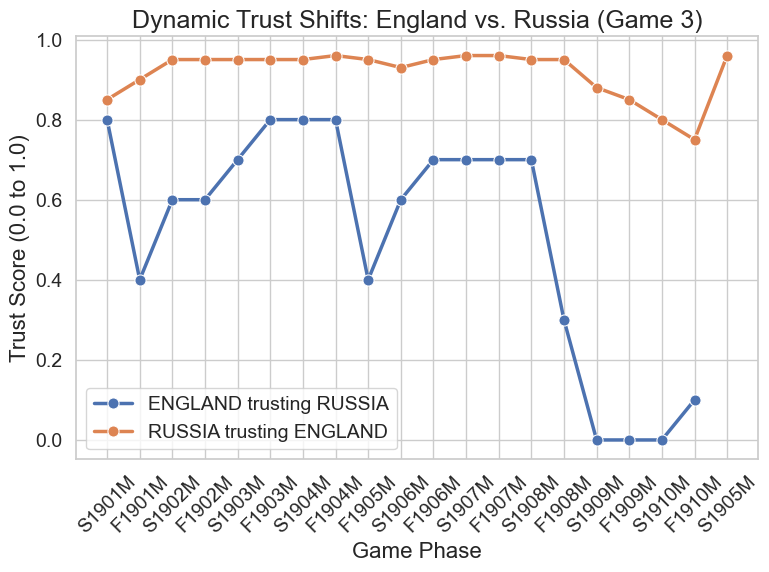
\includegraphics[width=\textwidth]{images/dynamic_trust_shifts.png}
        \phantomcaption
        % \caption{Micro Dynamics: England's internal trust in Russia drops to 0.0 prior to a betrayal, while Russia remains unaware.}
        \label{fig:trust_shift}
    \end{subfigure}
    \hfill
    % Second Subfigure: The Macro View (Global Alliances)
    \begin{subfigure}[b]{0.48\textwidth}
        \centering
        % Replace with your actual filename
        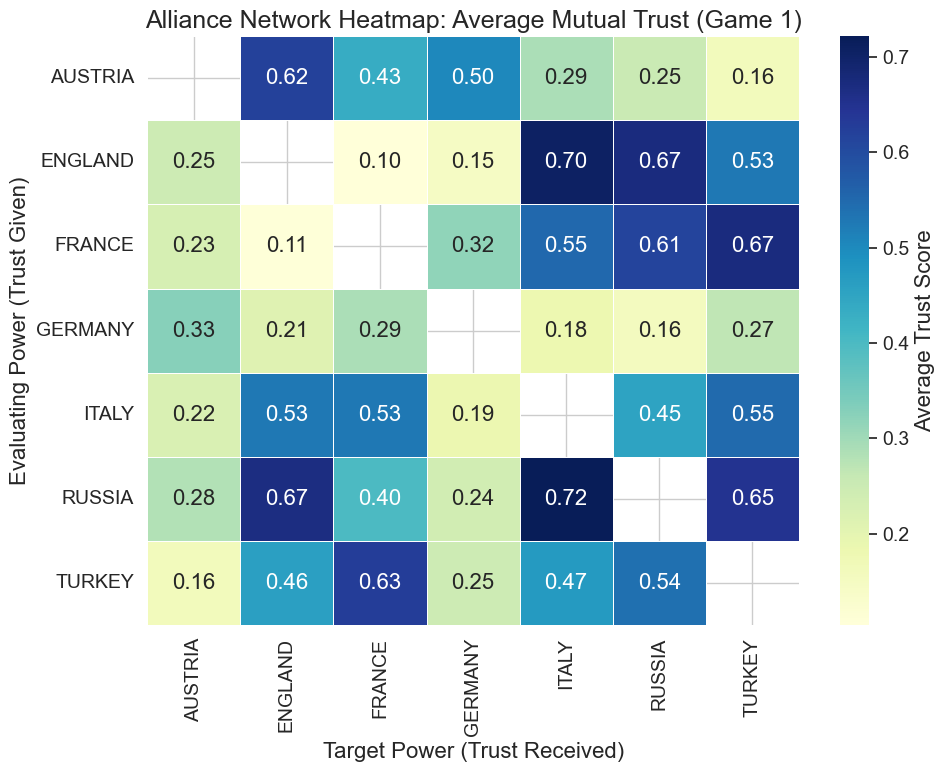
\includegraphics[width=\textwidth]{images/alliance_heatmap.png} % Ensure this matches your heatmap filename
        \phantomcaption
        % \caption{Macro Dynamics: A trust matrix from Game 1 successfully maps overarching geopolitical alliances and isolated pariahs.}
        \label{fig:trust_heatmap}
    \end{subfigure}
    
    \caption{Core Capabilities of the LLM Trust System. The system captures localized, asymmetrical deception (left) while simultaneously generating coherent, board-wide diplomatic networks (right).}
    \label{fig:trust_summary_panel}
\end{figure}

\subsection{Results}
The following findings were derived from our first experiment, which evaluated the core trust system's behavior in "naive" agents. This established a baseline control group, allowing us to accurately isolate and measure the impact of the cross-game memory loops in subsequent experiments.

\textbf{Dynamic Deception \& The Sucker's Metric:} Continuous tracking of mutual trust scores successfully quantified diplomatic backstabs. In Game 3, England and Russia maintained high mutual trust (0.7--0.9) until 1908, when England's internal trust in Russia plummeted to 0.0 ahead of a betrayal \bref{fig:trust_shift}. Russia remained unaware, maintaining a 0.88 trust score. This visually proved the framework captures unilateral alliance breakdowns. Other extreme asymmetries included massive trust gaps of 0.95 (Game 1) and 0.90 (Game 2).

\textbf{Trust vs. Game Success:} Comparing average received trust against final supply centers revealed no meaningful correlation ($r = -0.05$), proving that universally trusted agents do not inherently win. Victory relies on tactical positioning and timely betrayals rather than simply projecting honesty. Additionally, we observed no strong "Paranoia Effect" ($r = 0.12$): agents that frequently perceived betrayal did not systematically withdraw trust across the board.

\textbf{Global Alliance Mapping:} By aggregating mutual trust scores into matrices, the system successfully mapped overarching geopolitical landscapes. Trust heatmaps from Game 1 clearly visualized strong mutual axes (England-Russia), isolated pariahs (Germany, Austria), and agents successfully playing multiple sides (Italy) \bref{fig:trust_heatmap}.

\textbf{LLM Personas \& Adaptation:} Underlying architectures strictly dictated baseline diplomatic postures. Grok (\texttt{x-ai/grok-4.1-fast}) emerged as the most cooperative baseline (0.54), while Qwen variants were highly skeptical ($\sim$0.33--0.42). However, these personas were not static. Progression tracking showed dynamic adaptation, with almost all models exhibiting a sharp, widespread decline in given trust during the late game (1908-1910) as board tensions peaked \bref{fig:model_adaptation}.

\textbf{The Instruction-Following Artifact:} Analysis of unprompted trust score updates revealed a massive architectural artifact rather than pure strategic paranoia. Models like Grok, Qwen, and GPT-OSS frequently failed to document their internal reasoning, making nearly 100\% of their updates appear unprompted due to JSON schema adherence failures. Conversely, models like Claude and Gemini meticulously populated these textual evidence fields. Furthermore, this failure to document reasoning showed virtually no correlation ($r = -0.05$) with final game success.

\begin{figure}[htbp]
    \centering
    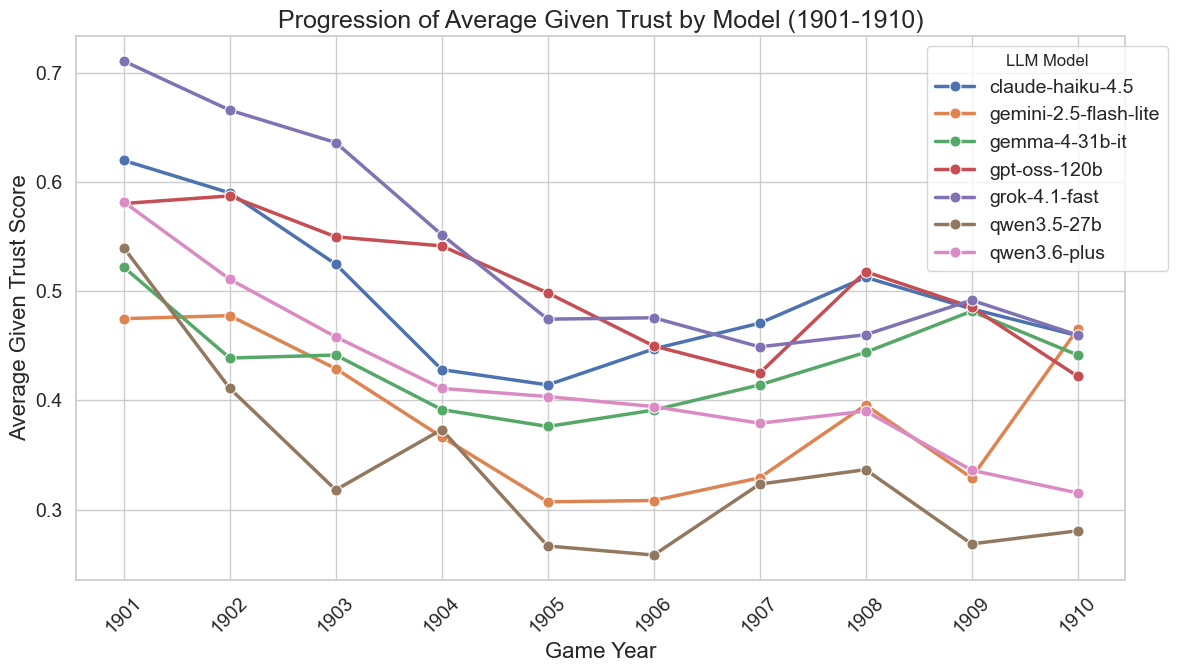
\includegraphics[width=0.85\textwidth]{images/model_trust_progression.png}
    \caption{Average Given Trust by Model (1901-1910): Highlights baseline architectural differences and a sharp late-game decline across most models.}
    \label{fig:model_adaptation}
\end{figure}

\clearpage
\section*{Ehrenwörtliche Erklärung}

Ich versichere, dass ich die beiliegende Bachelor-, Master-, Seminar-, oder
Projektarbeit ohne Hilfe Dritter und ohne Benutzung anderer als der angegebenen
Quellen und in der untenstehenden Tabelle angegebenen Hilfsmittel angefertigt
und die den benutzten Quellen wörtlich oder inhaltlich entnommenen Stellen als
solche kenntlich gemacht habe. Diese Arbeit hat in gleicher oder ähnlicher Form
noch keiner Prüfungsbehörde vorgelegen. Ich bin mir bewusst, dass eine falsche
Erklärung rechtliche Folgen haben wird.

% Declare below which AI tools you used in the process of writing your work,
% including text, image, code, and data generation. If you used a tool for a
% purpose not included in the list yet, add it to the list.
\begin{center}
  \textbf{Declaration of Used AI Tools} \\[.3em]
  \begin{tabularx}{\textwidth}{lXlc}
    \toprule
    Tool & Purpose & Where? & Useful? \\
    \midrule
    ChatGPT & Rephrasing & Throughout & + \\
    DeepL & Translation & Throughout & + \\
    ResearchGPT & Summarization of related work & Sec.~\ref{sec:related_work} & - \\
    Dall-E & Image generation & Figs.~2, 3 & ++ \\
    GPT-4 & Code generation & functions.py & + \\
    ChatGPT & Related work hallucination & Most of bibliography & ++ \\
    \bottomrule
  \end{tabularx}
\end{center}

\vspace{2cm}
\noindent Unterschrift\\
\noindent Mannheim, den XX.~XXXX 2024 \hfill

\end{document}